The lexer can recognize the following number formats:
\begin{itemize}[noitemsep]
    \item Decimal numbers (e.g. \textcolor{teal}{42}) 
    \item Hexadecimal numbers (e.g. \textcolor{teal}{Ex2A})
    \item Real numbers (e.g. \textcolor{teal}{3.14})
    \item Babylonian numbers (e.g. \textcolor{teal}{ EB\{YY \textless{\textless}\}BE })
\end{itemize}
\noindent
Decimal and Real numbers can be used in code in the expected way. Hexadecimal numbers
need to be escaped with the \textcolor{teal}{Ex} prefix.\newline
While the first three are self-explanatory, the Babylonian numbers are a bit more complicated.
They can be used in code like this: 
\begin{center}
    \textcolor{teal}{ EB\{insert\_babylonian\_number\_here\}BE }
\end{center}
\noindent
The Babylonian number is then converted to a decimal number by the lexer.
Valid characters for the babylonian numbers are:
\begin{itemize}[noitemsep]
    \item \textcolor{teal}{Y} equals 1
    \item \textcolor{teal}{\textless} equals 10
    \item Empty space is delimiter for the digits
\end{itemize}
\noindent
The babylonian number system is a positional number system, where the base is 60.
The following table show the representation of the numbers 1 to 59:
%include picture and give add Babylonian as source
\begin{center}
    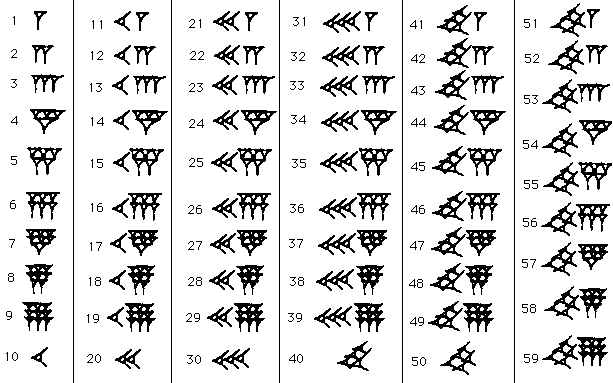
\includegraphics[width=0.5\textwidth]{babylonian_numbers.png}
    \cite{Babylonian}
\end{center}
\noindent







